% !TeX spellcheck = en_US

\chapter{Background}
\label{chp:background}

	In this chapter, we provide background information for our paper to give the reader a better understanding of our work. We explain used terminology in \autoref{sec:terminology} and give an overview of the extension architecture that we focus on in \autoref{sec:extensionArchitecture}.

\section{Terminology}
\label{sec:terminology}

\paragraph{Browser}

	A browser is a desktop application to display web pages. It executes HTTP requests to fetch web pages from remote hosts and allows the user to interact with them. Furthermore, the browser executes JavaScript embedded into a web page which allows a dynamic interaction and changes the web pages look according to Cascading Style Sheets (CSS).
	
\paragraph{Browser Plugin}
	
	A browser plugin is an external application that runs on the hosting system. It commonly provides an API or a graphical user interface that is embedded into a web page on demand. We do not cover plugins in this paper.
	
\paragraph{Browser Extension}
	
	A browser extension is an additionally piece of software that enhances a browser's functionality or user interface. Unlike browser plugins, it is considered as a part of the browser itself. Therefore, it has access to some features of the browser such as cookies or bookmarks and can modify displayed web pages. 

\paragraph{Web Application}

	A web application is a server-client software application, hosted on a remote server and accessible for the user using the HTTP or HTTPS protocols.

\paragraph{Document Object Model (DOM)}

	The \textit{Document Object Model} is a standardized API for representing HTML or XML documents as a tree \cite{w3cDOMSpecification}. This allows scripting languages, such as JavaScript, to easily manipulate the document's content. It is used by browsers to internally store web pages and can be accessed by JavaScript through the \texttt{document} object. 

\paragraph{XMLHttpRequest (XHR)}

	The XMLHttpRequest API allows JavaScript to programmatically execute HTTP and HTTPS requests. It is often used to load dynamic content or to transfer information to a server. 

\paragraph{Same Origin Policy (SOP)}
	
	The \textit{Same Origin Policy} is a browser security policy that isolates web pages with different \textit{origins} from each other. The origin of a web page is defined by the scheme, host, and port of its URL \cite{w3cOriginSpecification}. The browser permits scripts to access the content of another web page only if both have the same origin. Whereas, the origin of a script is defined by the origin of the web page that it is embedded into and not the origin from where the script was fetched. This policy prevents malicious scripts to access sensitive information from another web page and to execute requests to cross-origins. 
	
	A simple scenario shows why this policy is an important and efficient tool to secure the user's privacy. If a user authenticates to a web application such as an online banking platform, a cookie that contains a unique identifier is often stored inside the user's browser. The cookie is send along any request to the web application and authenticates the user on each request. Without the SOP, a malicious script within another browser tab could send a valid request to the application because the authentication cookie is sent along the request. The script could fetch a secured web page from the application and read out the user's sensitive information or perform a request to execute an action on behalf of the user such as to execute a banking transfer.  
	
\paragraph{Content Security Policy (CSP)}

	The \textit{Content Security Policy} is another browser security policy that restricts the sources from which the web page is allowed to fetch its resources \cite{w3cContentSecurityPolicySpecification}. Unlike the SOP, which restricts all web pages, the CSP has to be declared by the web page's author. It is intended to reduce the attack surface in the case that an attacker has successfully compromised the web page. By explicitly declaring origins from which the web page is allows to fetch resources, the attacker is hampered because he is not able fetch additional malicious content from his server. Furthermore, the CSP disables the use of \textit{eval} and related functions such as \texttt{setTimeout(string, number)}, \texttt{setInterval(string, number)}, and \texttt{new Function(string)} and it disables inline JavaScript (\texttt{<script>...</script>}) and inline event handler (\texttt{<button onclick="...">}).
	
	A CSP consists of several directives and corresponding values delimited by a semicolon. A directive declares the restriction for a particular resource type such as scripts, styles, or images. The corresponding values declare origins from which the web page is allowed to load the resources. They may either be a URL with wildcards to match several origins at once, \texttt{'none'}, or \texttt{'self'}. The \textit{none} key disables the loading of the resource from any origin and the \textit{self} key restricts it to the web page's origin. To remove the additional restriction on eval, the web page's developer may add the key \texttt{'unsafe-eval'} to the script directive and to remove the additional restriction on inline scripts, the developer may add the key \texttt{'unsafe-inline'} to generally allow inline scripts. A more fine-grained tuning can be achieved by a nonce or hash. A nonce is randomly generated value that is declared in the script directive and enables any script element that has a \textit{nonce} attribute containing the same random value. Similar, adding the computed hash value of a script to the script directive enables the execution of this script. Both approaches do not work for inline event handler.
	
	The following example shows a valid CSP:
	\begin{center}
		\texttt{default-src 'self'; script-src 'self' https://trusted.server.com/* 'unsafe-eval';}
	\end{center}
	First, we set the default directive and therewith restrict all other directives to the origin of the underlying web page. Next, we lighten the restriction to load scripts from a trusted server and allow the use of eval in loaded scripts.

\newpage
\section{Extension Architecture}
\label{sec:extensionArchitecture}

	In the past, each browser had its own architecture for extensions. This led to an additional workload for a developer, if he wanted his extension to be compatible with multiple browsers. He had to implement an extension for each browser, even though each provides equal functionality. Nowadays, the browsers' developers seem to address this unhandy situation and started to use a cross-browser extension architecture. In our paper, we focus on this architecture which is supported by Google's \textit{Chrome} browser, Mozilla's \textit{Firefox} browser, Microsoft's \textit{Edge} browser, and the \textit{Opera} browser. We have analyzed the extension's structure in-depth and provide our results in this section.

	The cross-browser extension architecture is based on a research described earlier in \autoref{sec:relatedWorks:extensionArchitecture}. The researchers examined the model of Firefox's Add-ons and revealed many vulnerabilities in connection to Add-ons running with the user's full privileges. This enables an attacker, in the case that he has compromised the Add-on, to access arbitrary files and launch new processes. To counter the found exploits, the researchers proposed a new model that should protect the user from unintentionally implemented vulnerabilities.

	The developers of Google's Chrome browser where the first to adapt the proposed model in 2010. In 2013, the developers of the Opera browser switched the browser's underlying framework to \textit{Chromium} which is also the framework for Chrome \cite{operaBlogSwitchToChromium}. With this change, they adopted the same extension architecture that Chrome uses. In 2015, the developers of Mozilla's Firefox browser announced that they will support the extension model, too. They published a first version of their implementation in version 42 of Firefox. Currently, their implementation is still being developed and therefore not all browser APIs are supported \cite{mozillaWebExtensionStatus}. Similar, Microsoft started in 2016 to implement the same architecture for their new Edge browser and the support for many browser APIs is currently still in development \cite{edgeBrowserApiStatus}.

\subsection{General Structure}

	Extensions implemented in the cross-browser architecture use only web technologies such as JavaScript, HTML, and CSS. All included files are declared in a mandatory manifest which also holds the extension's meta information such as its name, version, and author. \autoref{code:manifest} shows an example of a manifest file. 

	\begin{figure}[h]
		\begin{lstlisting}
{
	"manifest_version": 2,
	"name": "Extension Name",
	"version": "1.1.2",
	"background": {
		"scripts": [ "background.js" ]
	},
	"content_scripts": [ {
		{ 	"js": [ "content.js" ],
			"matches": [ "http://*/*", "https://*/*" ] }
	],
	"permissions": [ "cookies", "tabs", "http://*/*", "https://*/*" ],
	"content_security_policy": 
		"script-src 'self' https://*.example.com/ 'unsafe-eval'; object-src 'self'"
}
\end{lstlisting}
		\caption{Example \texttt{manifest.json} file.}
		\label{code:manifest}
	\end{figure}
	
	The extension's general structure, as shown in \autoref{fig:extensionArchitectureStructure}, is divided into the background that holds the extension's main logic including user interfaces and content scripts that are used to interact with web pages.
	
	\begin{figure}[h]
		\centering
		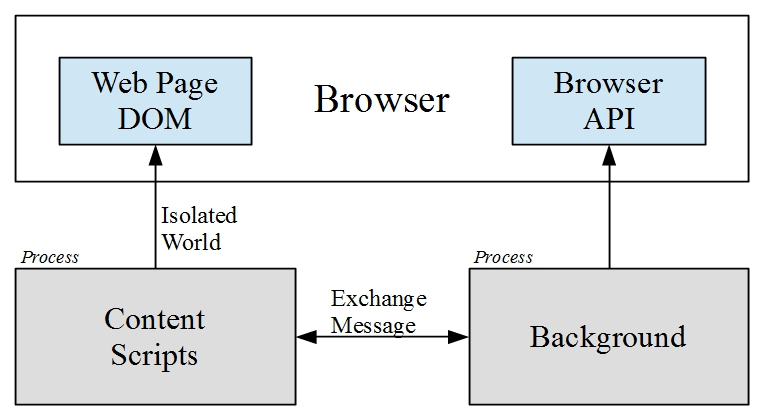
\includegraphics[width=0.7\textwidth]{./graphics/extension_overview.png}
		\caption{Structure of the cross-browser extension architecture.}
		\label{fig:extensionArchitectureStructure}
	\end{figure}
		
	
\subsubsection{Background Page}

	The \textit{background page} is a HTML document invisible for the user which includes JavaScript code that controls the extension's behavior. The extension that uses the manifest shown in \autoref{code:manifest}, declares a single JavaScript file that is added to its background page on line 4. From within the background page, the extension has access to additional functionality provided by a browser API such as access to the browser's tab-system, the possibility to observe and intercept web requests, or the access to the user's bookmarks. In order to use some of the browser API modules, the extension has to declare a corresponding permission in its manifest. Similar, in order to access a remote server using a web request or accessing a tab that contains a web page, the extension has to declare a host permission that matches the target's URL. A host permission is a URL pattern that may contain wildecards for the scheme, domain, or path to match several web pages at once. For example, the URL pattern \texttt{http://*.example.com/*} matches \texttt{http://api.example.com/} and \texttt{http://www.example.com/foo} but not \texttt{https://www.example.com/} and \texttt{http://www.example.org/}. The example manifest file shown in \autoref{code:manifest} declares the \texttt{cookies} and \texttt{tabs} permissions and host permissions for all web pages using the two URL pattern \texttt{http://*/*} and \texttt{https://*/*}.	
	
	Additionally, a developer can declare the access to API modules that are not required for his extension's basic functionality as optional permissions. If the extension requests access to an optional API module at runtime, the browser prompts the user to confirm the request. A confirmed optional permission stays active even after a browser restart until the extension itself removes it. Furthermore, host permission may also be declared as optional which gives the user a fine-grained tuning of websites to which an extension has access to. 
	
	An extension may include additional user interface elements such as pop-up or option pages. JavaScript inside a user interface has direct access to the background page which allows it to invoke methods and access variables of it and vice versa. 
	
\subsubsection{Content Scripts}
	
	A extension can not directly access a web page or its DOM from within its background. For that purpose, it uses content scripts which have full access to the DOM of a single web page in whose context they are active. This allows the extension to extract values from the web page or to modify its content. Content scripts are very limited in their access to the browser's API. They can only use a small subset of modules such as the internationalization or the storage module. Furthermore, the background and a content script can not directly interact with each other. They can only use a JSON-based communication channel to transfer commands or data between each other. 
	
	Next to the programmatically injection of a content script into a tab from within the extension's background, the developer can also register the content script in the extension's manifest. To determine the web pages in which the content script will be active, the developer has to add a URL pattern. In contrast to the programmatically injection which needs a valid host permission to access the tab, the statically registered content scripts do not need additional permissions. In the manifest shown in \autoref{code:manifest}, the extension registers a single JavaScript file on line 7. It will be active in any web page whose URL matches \texttt{http://*/*} and \texttt{https://*/*}.
	
	A content script underlies almost the same restriction as a web page. The Same Origin Policy that restricts a script to access another origin than its own applies partly to a content script. If the web page contains an iframe element from a cross-origin, the content script that runs in the main web page can not access the iframe's content. The iframe is handled as separate web page which means that another content script may be active in its context. The SOP also restricts web requests to cross-origins. But here exists a exception for content scripts because they are allowed to execute programmatically executed web requests using a XMLHttpRequest. The request is only restricted by the extension's host permissions but not by the SOP. 

\subsection{Security Features}

	The researchers that designed the cross-browser extension architecture focused to improve the security of the extension's user. They developed the architecture under the assumption that many extension developers are merely hobby developers and not security experts and therefore may unintentionally implement vulnerabilities \cite{Barth10protectingbrowsers}. The extension architecture underlies several security features which we present in the following list.
	
\begin{itemize}		
	\item[\textbf{Component Separation}] To hamper an attacker who has compromised one component of an extension, the extension's components are strictly separated from each other. The extension's background and content scripts run in their own process on the host's operating system. This creates an efficient boundary between the components because they do not share a common memory section and therefore are not able to invoke methods or access variables of each other. If an attacker has compromised one component of the extension, he can only access the other through the JSON-based message channel. If the extension's developer did not create a vulnerability at the other side of the communication channel, the attacker is not able to compromise the rest of the extension. 
	
	\item[\textbf{Isolated World}] Because content scripts are exposed to potential attacks from malicious web pages, they underly an additional security feature called \textit{Isolated World}. Content scripts and the JavaScript inside the web page run in their own process on the operating system. Consequently, they are not able to access methods or variables of each other. Furthermore, content scripts have their own instance of the \texttt{document} object mirroring the web page's DOM that is natively stored inside the browser. If a script modifies the DOM, each instance is updated accordingly. However, if a script overrides a DOM method or adds a non-standard property to its \texttt{document} object, the changes will not be transferred to the internally stored DOM and consequently not to other instances of the \texttt{document} object, too. \\	
	This mechanism effectively shields content script from \textit{cross-origin JavaScript capability leak} attacks that try to manipulate the behavior of JavaScript methods used by the content script \cite{Carlini:2012:EGC:2362793.2362800, Barth:2009:CJC:1855768.1855780}. Furthermore, if a content script inserts untrusted HTML code into a web page's DOM, for instance setting the \texttt{innerHTML} property of a DOM element, any code inside the content will be executed inside the web page's separated process instead of the content script's process. Thus, the strict separation prevents potential XSS attacks against the extension that the developer may has added unintentionally.

	\item[\textbf{Permissions}] The permission system is not only intended to get a lead of the extension's capabilities and purpose, but also acts as a security feature to reduce the attack surface in the case that an attacker has compromised the extension. It works with the principle of least privileges. An extension has by default access to no API modules and origins. Only if it declares a permission it is granted access to the corresponding privilege. An attacker is also restricted by this constraints. He is not able to access other privileges than the declared ones. 
	
	\item[\textbf{Content Security Policy}] To reduce the threat of potential cross-site scripting attacks, the background page underlies a Content Security Policy. The default CSP consists of the directives \texttt{script-src 'self'} and \texttt{object-src 'self'}. This limits the loading of scripts and other resources to files from within the extension's bundle. Additionally, it disables the use of \texttt{eval} and inline scripts. \\
	A developer may relax or tighten the policy for his extension by declaring a custom CSP in the extension's manifest which has to contain at least the \textit{script} and \textit{object} directives. Adding the URL of a remote origin to the CSP allows to fetch resources from the declared host. Again, an URL pattern may be used to match several hosts at once, but wildcards are only allowed for the subdomain. To ensure that remotely loaded resources have not been replaced or modified by a network attacker, only origins that use a secured connection such as HTTPS are allowed. If the developer wishes to use \texttt{eval} or related functions in his extension's background page, he has to add the value \texttt{'unsafe-eval'} to the \textit{script} directive. If he wishes to use inline scripts, he has to add the hash value of the script to the script directive. The \texttt{'unsafe-inline'} key is not allowed and therefore the execution of inline event handler can not be enabled. \\
	The manifest shown in \autoref{code:manifest}, declares a custom CSP on line 13. It enables the loading of remote scripts from any URL that matches \texttt{https://*.example.com/} and enables the user of \texttt{eval} in the background page.

	\item[\textbf{Privacy Preserving Measures}] The security features described before aim to protect the user from an attacker who tries to compromise the extension. They do not protect the user from intentionally implemented malicious behavior. However, some features exist protecting the user's privacy, if used correctly. These features reduce the privileges an extension has by default and give the user the possibility to explicit grant the extension further privileges. \\
	The \texttt{activeTab} permission gives an extension temporary access to the currently active web page if the user explicitly invokes the extension. This occurs if the user clicks an interface element that belongs to the extension such as a button in the browser's toolbar or an entry in the web page's context menu. The extension will lose the access to the web page as soon as the tab loads another web page or is closed. This feature is intended to reduce the amount of needed permissions for extensions that only interact with the current web page and only on the user's demand. Otherwise, those extensions would need full and persistent access to any web page to be able to act if the user invokes them. \\
	Similar to the \texttt{activeTab} permission, the extension's developer can declare permissions as optional. This declares the permissions as not necessary for the extension's base functionalities but they provide additional features on the user's demand. If the extension requests an optional permission, the browser prompts the user to confirm. Even host permissions may be declared as optional, allowing the user to fine-grained control the extension's access to web pages. However, the extension has to remove the requested permission itself. If not, the permission stays active until the extension is uninstalled. The user can not remove an accepted permission by himself if the extension does not provide a proper interface. 
	
\end{itemize}

\subsection{Comparison}
	
	We have analyzed the extension architectures of Firefox Add-ons and Safari extensions. In this section, we present their structure and some of their security features and compare them with the cross-browser extension architecture.

\subsubsection{Firefox Add-ons}
	
	Firefox's support for the multi-browser extension model is currently still in development \cite{mozillaWebExtensionStatus}. Therefore, extensions implemented in the old Add-on model are still in use. 
	
	Mozilla distributes Add-ons through their own web store\footnote{\url{https://addons.mozilla.org/en-US/firefox/}} but also allows the installation from other sources. Add-ons published through the web store are the target of a review by Mozilla's security experts \cite{mozillaDevReviewPolicy}. After passing the review, the Add-on is signed by Mozilla what is shown on installation to the user. If an Add-on is published private and was not the target of a successful review, it is labeled as untrusted on installation. 
	
	To develop an Add-on, an additional JavaScript framework distributed by Mozilla is necessary. It contains several core modules that encapsulate the functionality that the browser provides to the Add-ons similar to the browser's API of cross-browser extensions. Additionally, the \texttt{chrome} module even provides full access to browser-internal functionality including the access to the underlying host system. To use a module, the Add-on has to explicit include it in its source code using the global function \texttt{require} that takes the module's name as parameter. 
	
	Firefox uses a security mechanism that is comparable with the cross-browser extensions' permission system. It serves the same purpose to reduce an attackers scope of action if he managed to compromise the extension. On compiling the Add-on, a scanner retrieves all calls of \texttt{require} from the Add-on's source code and lists all requested modules. The runtime loader will actually prevent the loading of modules that are not listed. Furthermore, the list of requested module is primarily used by Mozilla's reviewers to get a hint of the extension's purpose and capabilities. If an Add-on requires for example the \texttt{chrome} module that gives access to the browser's internal functionality which includes, among others, full access to the host system, the Add-on is subject to an extra in-depth security review. However, contrary to cross-browser extensions, the user does not get notified if the Add-on requests a particular module.
	
	In their framework, Firefox's developers have adapted the separation between the extension's core and content scripts like the cross-browser extensions use it. The \texttt{page-mod} module provides the functionality to execute scripts in the scope of a web page. However, this separation is not complete because the \texttt{window/utils} module still provides a function to directly access the web page's \texttt{window} object.  \\
	Furthermore, the Add-ons components are not as strictly separated as the components of a cross-browser extension. Where each content script and the extension's background run in its own process on the operating system, Firefox uses a programmatically solution to separate the Add-ons content. They wrap untrusted content such as web pages and provide only a filtered view to the Add-on. An attacker is more likely to expose a vulnerability in the wrapping implementation than he is able to bypass the process boundary between the contents of a cross-browser extension because he has no access to the hosting system.
	
	In conclusion, the Add-on architecture has less build in security features and provides more functionality than the cross-browser extension architecture. This increases the danger of compromised Add-ons because an attacker is less restricted in his actions and is able to harm the user more than with a compromised cross-browser extension. The fact that each Add-on published over the web store is targeted by a security review decreases the danger from malicious and vulnerable implemented Add-ons, but user are still able to install not-reviewed Add-ons from other sources. 
	
\subsubsection{Safari Extensions}

	Compared to other extension models, Safari extensions are very limited in their capabilities. The browser provides almost no functionality and therefore extension's are restricted to the interaction with web pages. This increases the user's privacy at least partly because an extension can not access information stored inside the browser such as bookmarks or the browsing history. But still, most sensitive information are stored inside web pages. 
	
	To publish an extension, the developer needs a certificate provided by Apple. This ensures that only registered developers are able to publish extensions which hampers the distribution of malicious extensions. If a certificate is invalid, Safari will disable the developer's extensions.
	
	The browser facilitates the extension development by providing a build-in user interface. It manages the extension's content such as meta information or source code files.	An additional feature allows to define content that will be blocked in web pages. The extension's developer can add content-blocking rules to his extension that are compiled into a byte-code format and processed directly at runtime. This renders the programmatically examination of a web page's content and determination of blocking unnecessary and therefore provides a better performance \cite{safariContentBlockingRules}.
	
	In conclusion, Safari extensions compared to the other extensions can do the least harm to the user because of their limited capabilities. Furthermore, the needed certificate hampers developers to intentionally distribute malicious extensions.